
% header %{{{1

\documentclass[tikz, border=1mm]{standalone}

\usepackage{amsmath}

\usepackage{tikz}

\usetikzlibrary{calc,angles,quotes,shapes.geometric}

\usepackage{tkz-euclide}

% document %{{{1

% opening %{{{2

\begin{document}
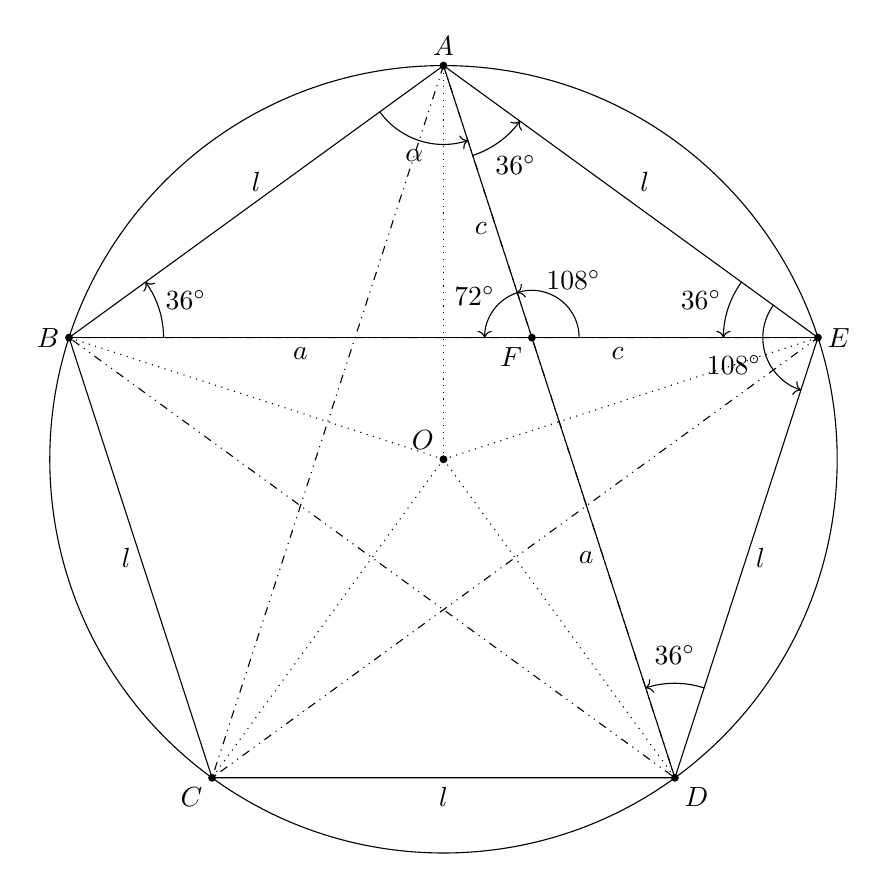
\begin{tikzpicture}[scale=1.0]

% parameters %{{{2

	\def\numsides{5}
	\def\radius{5}
	\def\rotation{90}

% coordinates %{{{2

	\coordinate (O) at (0,0);
	\draw (O) circle (\radius);

	\foreach \i in {1,...,\numsides} {
		\coordinate (P\i) at ({360/\numsides*(\i-1)+\rotation}:\radius);
	}

% intersections %{{{2

	\tkzInterLL(P2,P5)(P1,P4)\tkzGetPoint{F}

% pentagon %{{{2

	\draw (P1) \foreach \i in {2,...,\numsides} { -- (P\i) } -- cycle;

% radiuses %{{{2

	\foreach \i in {1,...,\numsides} { \draw[dotted] (O) -- (P\i); }

% pentagram %{{{2

	\draw[dashdotdotted] (P1) -- (P3) -- (P5) -- (P2) -- (P4) -- cycle;
	\draw[solid] (P5) -- (P2);
	\draw[solid] (P1) -- (P4);

% points, dots, vertices %{{{2

	\fill (O) circle (0.5mm);
	\fill (F) circle (0.5mm);
	\foreach \i in {1,...,\numsides} { \fill (P\i) circle (0.5mm); }

% points, dots, vertices labels %{{{2

	\node[above left] at (O) {$O$};
	\node[below left] at (F) {$F$};

	\node[above] at (P1) {$A$};
	\node[left] at (P2) {$B$};
	\node[below left] at (P3) {$C$};
	\node[below right] at (P4) {$D$};
	\node[right] at (P5) {$E$};

	\node[above] at ($(P1)!0.5!(P2)$) {$l$};
	\node[left] at ($(P2)!0.5!(P3)$) {$l$};
	\node[below] at ($(P3)!0.5!(P4)$) {$l$};
	\node[right] at ($(P4)!0.5!(P5)$) {$l$};
	\node[above right] at ($(P5)!0.5!(P1)$) {$l$};

	\node[below] at ($(P2)!0.5!(F)$) {$a$};
	\node[left] at ($(F)!0.5!(P4)$) {$a$};
	\node[below] at ($(F)!0.3!(P5)$) {$c$};
	\node[left] at ($(P1)!0.6!(F)$) {$c$};

% angles labels %{{{2

	\pic[draw, ->, "$36^\circ$", angle radius=1.2cm, angle eccentricity=1.3]
	{angle = P5--P2--P1};

	\pic[draw, ->, "$36^\circ$", angle radius=1.2cm, angle eccentricity=1.3]
	{angle = P1--P5--P2};

	\pic[draw, ->, "$36^\circ$", angle radius=1.2cm, angle eccentricity=1.3]
	{angle = P4--P1--P5};

	\pic[draw, ->, "$36^\circ$", angle radius=1.2cm, angle eccentricity=1.3]
	{angle = P5--P4--P1};

	\pic[draw, ->, "$108^\circ$", angle radius=0.6cm, angle eccentricity=1.5]
	{angle = P5--F--P1};

	\pic[draw, ->, "$108^\circ$", angle radius=0.7cm, angle eccentricity=1.6]
	{angle = P1--P5--P4};

	\pic[draw, ->, "$72^\circ$", angle radius=0.6cm, angle eccentricity=1.5]
	{angle = P1--F--P2};

	\pic[draw, ->, "$\alpha$", angle radius=1.0cm, angle eccentricity=1.2]
	{angle = P2--P1--F};

% closing %{{{2

\end{tikzpicture}
\end{document}
